\chapter{Chi-Squared \(\chi^2\) Tests}
\section{The \(\chi^2\)-Distribution}
\begin{definition}{}{}
  A random variable \(X\) is said to follow a \(\chi^2\)-distribution, with degree of freedom \(\nu\), iff its probability density function is given by
  \[f(x)=\begin{cases}
    \frac{1}{2^{\nu/2}\Gamma(\nu/2)}x^{(\nu/2)-1}e^{-x/2} &\text{if \(x>0\)},\\
    0 &\text{otherwise}.
  \end{cases}\]
\end{definition}
\begin{figure}[H]
  \centering
  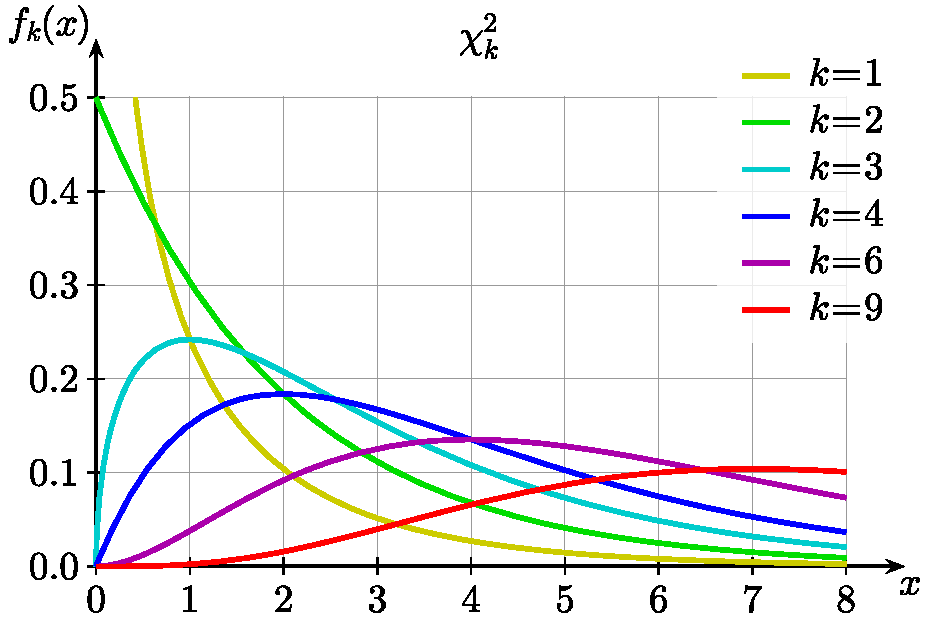
\includegraphics[width=0.7\textwidth]{../Diagrams/Chi-square.pdf}
  \caption{\ref{source:chi-squared} Illustration of how the \(\chi_{(\nu)}^2\) distribution looks with increasing degree of freedom \(\nu\).}
  \label{fig:chi-square}
\end{figure}
\begin{stbox}{General Information}
  \begin{itemize}
    \item Properties of chi-squared distributions.
    \begin{itemize}
      \item \(\E(X)=\nu\) and \(\Var(X)=2\nu\).
      % , and the mode of \(X\) is \(\max\{k-2,0\}\).
      \item The \(\chi_{(\nu)}^2\) distribution tends to a normal distribution as \(\nu\to\infty\).
      \item Suppose \(Z_i\sim\Normal(0,1)\) are independent. Then, \(Z_1^2+\dots+Z_n^2\sim\chi^2_{(n)}\).
      \item If \(X\sim\chi_{(\nu)}^2\) and \(Y\sim\chi_{(\upsilon)}^2\), then \(X+Y\sim\chi_{(\nu+\upsilon)}^2\).
    \end{itemize}
  \end{itemize}
\end{stbox}
\section{A Goodness-of-Fit Test}
\begin{stbox}{General Information}
    \begin{enumerate}
      \item Let [\(X\) in context].
      \item \emph{Note.} Use a pen to draw any necessary tables.

      \begin{tabular}{|ll|}
        \hline
        Test & \(H_0\colon\text{[\(X\) follows the distribution in context]}\)\\
        against &\(H_1\colon\text{[\(X\) does not follows the distribution in context]}\)\\
        \multicolumn{2}{|l|}{at the \(100\alpha\%\) significance level.}\\
        \hline
      \end{tabular}
      \item ~
      \begin{table}[H]
        \centering
        \begin{tabular}{|Sc|Sc|Sc|Sc|Sc|}
          \hline
          \(x\) & \(\leq x_1<\) & \(\leq x_2<\) & \(\cdots\) & \(\leq x_n<\)\\
          \hline
          \(f_i\) & \(f_1\) & \(f_2\) & \(\cdots\) & \(f_n\)\\
          \hline
          \(e_i\) & \(e_1\) & \(e_2\) & \(\cdots\) & \(e_n\)\\
          \hline
          \(\dfrac{(f_i-e_i)^2}{e_i}\) & \(\dfrac{(f_1-e_1)^2}{e_1}\) & \(\dfrac{(f_2-e_2)^2}{e_2}\) & \(\cdots\) & \(\dfrac{(f_n-e_n)^2}{e_n}\)\\
          \hline
        \end{tabular}
        \caption{Observed and expected frequencies for a goodness-of-fit test}
        \label{table:goodness-of-fit-test}
      \end{table}
      \item Check whether \(e_i\geq 5\) for each of the \(n\) classes. If it isn't, we need to combine \emph{just enough} adjacent classes, till they do. Working-wise, use some underbraces/overbraces to indicate the combined values. 
      \item Under \(H_0\), the test statistic is
      \[\chi^2=\sum{\frac{(F_i-E_i)^2}{E_i}}\sim\chi_{(\nu)}^2.\]
      Here, \(n\coloneq\#\text{classes}\) and \(\nu=(\#\text{classes}-\#\text{estimated parameters})-1\).
      \item Continue as per usual, calculating the critical region \(\chi_{(\nu)}^2>\chi^2_{(\nu,1-\alpha)}\) or the \(p\)-value.
    \end{enumerate}
\end{stbox}
\begin{GCSkills}{}
  \begin{itemize}
    \item To find the value of \(\chi^2_{(\nu,1-\alpha)}\), which satisfies \(\Prob\left(X>\chi^2_{(\nu,1-\alpha)}\right)=\alpha\), we use the table in the \href{https://www.seab.gov.sg/docs/default-source/national-examinations/syllabus/alevel/2022syllabus/List_MF26_y22_sy.pdf}{MF26 formula sheet (Page 9)}. Unfortunately, there is no inverse \(\chi^2\) function available.
    \item For the \(p\)-value:
    \begin{center}
      \texttt{stat} \(\Longrightarrow\) \texttt{TESTS} \(\Longrightarrow\) \texttt{D:\(\chi^2\)GOF-Test\dots}
    \end{center}
  \end{itemize}
\end{GCSkills}
\begin{note}
  If \(X\) follows a \emph{discrete} uniform distribution, we must state it out in words. We cannot write \(X\sim\operatorname{U}(\mu,\sigma^2)\) as this would denote that \(X\) is a \emph{continuous} random variable. But if \(X\sim\Binom(n,p)\) (or \(X\sim\Poisson(\lambda)\), etc), then we can just denote it as such. 
\end{note}
\begin{example}{\(\#\text{estimated parameters}=0\)}{}
  Given \(X\sim\Normal(0,1)\) (note how the \emph{population parameters} that define the distribution are \emph{known}), the degree of freedom \(\nu=n-1\).
\end{example}
\begin{example}{\(\#\text{estimated parameters}=1\)}{}
  Consider when \(X\sim\Binom(m,p)\), such that the expected frequency for each of the \(n\) classes is at least 5, but we do not know the exact value of \(p\). So, we \emph{estimate} it according to the sample given. Then, the degree of freedom is \(\nu=n-1-1=n-2\).
\end{example}
\begin{example}{\(\#\text{estimated parameters}=2\)}{}
  Similarly, suppose \(X\sim\Normal(\mu,\sigma^2)\), such that the expected frequency of each of the \(n\) classes is at least 5, and the true values of \(\mu\) and \(\sigma^2\) are unknown. In this case, the degree of freedom \(\nu=n-2-1=n-3\). 
\end{example}
\begin{note}
  Consider when we are testing 
\begin{center}
    \begin{tabular}{|ll|}
      \hline
      Test & \(H_0\colon X\sim\Normal(\mu,\sigma^2)\)\\
      against &\(H_1\colon X\not\sim\Normal(\mu,\sigma^2)\)\\
      \multicolumn{2}{|l|}{at the \(100\alpha\%\) significance level.}\\
      \hline
    \end{tabular} 
\end{center}
So, we want to fill up the values of \(e_i\) below.
\begin{table}[H]
  \centering
  \begin{tabular}{|Sc|Sc|Sc|Sc|Sc|}
    \hline
    \(x\) & \(a_1\leq x< a_2\) & \(a_2\leq x< a_3\) & \(\cdots\) & \(a_n\leq x\leq a_{n+1}\)\\
    \hline
    \(f_i\) & \(f_1\) & \(f_2\) & \(\cdots\) & \(f_n\)\\
    \hline
    \(e_i\) & \cellcolor{yellow} \(e_1\) & \(e_2\) & \(\cdots\) & \cellcolor{yellow} \(e_n\)\\
    \hline
  \end{tabular}
  \caption{Observed and expected frequencies when testing goodness-of-fit with a normal distribution.}
  \label{table:gof-normal} 
\end{table}
Let the sample size \(\sum f_i\) be \(m\). Then, we should calculate \(e_1=m\Prob(\highlight[green!50]{-\infty}<X< a_2)\) and \(e_n=m\Prob(a_n\leq X\leq \highlight[green!50]{\infty})\), instead of \(e_1=m\Prob(\highlight[red!30]{a_1}\leq X< a_2)\) or \(e_n=m\Prob(a_n\leq X\leq \highlight[red!30]{a_{n+1}})\). Similarly, for goodness-of-fit tests with Poisson and Geometric distributions, we must also be careful in ensuring that we account for \emph{all} possible values which \(X\) can take on, in calculating \(e_i\).
\end{note}
\begin{note}
  Suppose we are given a question of the following form.

  \vspace{-0.5\baselineskip}\rule{20cm-137.0549pt}{0.05mm}

  Some context\dots 
  \begin{table}[H]
    \centering
    \begin{tabular}{|Sc|Sc|Sc|Sc|Sc|}
      \hline
      \(x_i\) & \(x_1\) & \(x_2\) & \(\cdots\) & \(x_n\)\\
      \hline
      \(f_i\) & \(f_1\) & \(f_2\) & \(\cdots\) & \(f_n\)\\
      \hline
    \end{tabular}
    \caption{Some data.}
    \label{table:some-chi-data}
  \end{table}
  \begin{enumerate}[label=(\roman*)]
    \item Show, at the \(100\alpha\)\% significance level, that the data does not support the hypothesis of \(X\sim\operatorname{Geo}(p)\) with \(p=0.5\).
    \item State how the test in (i) would have to be amended to test the hypothesis of a geometric distribution for an \emph{unspecified value of \(p\)}.
  \end{enumerate}

  \rule{20cm-137.0549pt}{0.05mm}
  Then, for (ii), two main changes have to be made:
  \begin{enumerate}
    \item Estimate the value of \(p\) by computing the sample mean \(\widebar{x}\) and letting \(p=1/\widebar{x}\).
    \item Adjust the degree of freedom from 4 to \(4-1=3\), as there is one more restriction, that the mean must agree.
  \end{enumerate}
  (The phrasing is similar for gof tests for other distributions; simply use the appropriate estimators for the unknown population parameters.)
\end{note}
\begin{note}
  The \(\chi^2\) goodness-of-fit test showed that there is strong evidence for \(X\sim\Poisson(\lambda)\). Suggest a possible reason.

  % \rule{20cm-137.0549pt-25pt}{0.05mm}
  % \vspace{0.5\baselineskip}
  \[s^2=\rule{0.5cm}{0.05mm} \qquad \widebar{x}=\rule{0.5cm}{0.05mm}\]
  Since \(\widebar{x}\approx s^2\), the population mean and population variance of the [\(X\) in context] may be approximately equal. This made the data a good fit to the Poisson distribution.
\end{note}
\begin{note}
  Explain why a test based on a normal distribution might still be valid, despite the \(\chi^2\) test-of-independence implying that \(X\not\sim\Normal(\mu,\sigma^2)\).
  \begin{enumerate}
    \item The sample size of \rule{0.5cm}{0.01mm} is small. Hence, the result of the test may not accurately represent the population.
    \item{} [\(X\) in context] might still be normally distributed, but with \(\E(X)\neq\mu\) and/or \(\Var(X)\neq\sigma^2\).
  \end{enumerate} 
\end{note}
\section{Tests of Independence}
\begin{stbox}{General Information}
  \begin{enumerate}
    \item Let [\(X\) in context].
    \item 
    \begin{tabular}{|ll|}
      \hline
      Test & \(H_0\colon\text{[\(X\) in context] is independent of [\(Y\) in context]}\)\\
      against &\(H_1\colon\text{[\(X\) in context] is dependent on [\(Y\) in context]}\)\\
      \multicolumn{2}{|l|}{at the \(100\alpha\%\) significance level.}\\
      \hline
    \end{tabular}
    \item \emph{Note}. Unless the question asks for it, we do not need to write \(\left[ \frac{(f_i-e_i)^2}{e_i} \right]\) or its corresponding values, in the following table.
    \begin{table}[H]
      \hypertarget{table:tests-of-indepedence}{}
      \centering
      \begin{tabular}{ScSc|Sc|Sc|Sc|Sc|Sc}
        \cline{1-6}
        % &&\multicolumn{4}{Sc|}{\(X\)}&\\
        % \cline{3-7}
        % && \(x_1\) & \(x_2\) & \(\cdots\) & \(x_n\) & \multicolumn{1}{Sc|}{Total}\\
        \multicolumn{2}{|Sc|}{\multirow{2}{*}{\(f_i\) \((e_i)\) \(\left[ \frac{(f_i-e_i)^2}{e_i} \right]\)}} &\multicolumn{4}{Sc|}{\(X\)}&\\
        \cline{3-7}
        \multicolumn{2}{|Sc|}{}& \(x_1\) & \(x_2\) & \(\cdots\) & \(x_n\) & \multicolumn{1}{Sc|}{Total}\\
        \hline
        \multicolumn{1}{|Sc|}{\multirow{4}{*}{\(Y\)}}&\(y_1\)&&&&&\multicolumn{1}{Sc|}{\(t_{r_1}\)}\\ 
        \cline{2-7}
        \multicolumn{1}{|Sc|}{}&\(y_2\)&&&&&\multicolumn{1}{Sc|}{\(t_{r_2}\)}\\ 
        \cline{2-7}
        \multicolumn{1}{|Sc|}{}&\(\vdots\)&&&&&\multicolumn{1}{Sc|}{\vdots}\\
        \cline{2-7}
        \multicolumn{1}{|Sc|}{}&\(y_m\)&&&&&\multicolumn{1}{Sc|}{\(t_{r_m}\)}\\  
        \hline
        \multicolumn{1}{Sc|}{}& Total & \(t_{c_1}\) & \(t_{c_2}\) & \(\cdots\) & \(t_{c_n}\) & \multicolumn{1}{Sc|}{\(S=\sum{t_{r_i}}+\sum{t_{c_i}}\)}\\ 
        \cline{2-7}
      \end{tabular}
      \caption{\emph{Expected} frequencies for a test of independence.}
      \label{table:tests-of-indepedence}
    \end{table}
    % \Bigg(The expected frequencies are given by \(e_{ij}=\dfrac{\text{row total}\cdot\text{column total}}{\text{total number of observations}}=\dfrac{t_{r_i}t_{c_j}}{S}\).\Bigg)
    \vspace{-1em}
    \begin{minipage}{0.825\textwidth}
      \begin{remark}
        \hypertarget{test-of-independence-expected-frequencies}{}
        The expected frequencies are given by \(e_{ij}=\dfrac{\text{row total}\cdot\text{column total}}{\text{total number of observations}}=\dfrac{t_{r_i}t_{c_j}}{S}\).
      \end{remark}
    \end{minipage}
    \item Check whether \(e_i\geq 5\) for each of the \(mn\) cells. If it isn't, we need to combine \emph{just enough} adjacent classes, till they do. Working-wise, use some underbraces/overbraces/side braces to indicate the combined values. 
    \item Under \(H_0\), the test statistic is
    \[\chi^2=\sum{\frac{(F_i-E_i)^2}{E_i}}\sim\chi_{(\nu)}^2.\]
    Here, \(n\coloneq\#\text{cols}\) and \(\nu=(\#\text{rows}-1)(\#\text{cols}-1)\).
    \item Continue as per usual, calculating the critical region \(\chi_{(\nu)}^2>\chi^2_{(\nu,1-\alpha)}\) or the \(p\)-value.
  \end{enumerate}
\end{stbox}
\begin{GCSkills}{}
  Key in the matrix of observed frequencies: 
  \begin{center}
    \texttt{2nd} \(\Longrightarrow\) \(\texttt{x}^{-1}\) \(\Longrightarrow\) \texttt{EDIT} \(\Longrightarrow\) \texttt{[A]}.
  \end{center}
  Then, conduct the test for independence:
  \begin{center}
    \texttt{stat} \(\Longrightarrow\) \texttt{TESTS} \(\Longrightarrow\) \texttt{C:\(\chi^2\)-Test\dots}
  \end{center}
\end{GCSkills}
\begin{note}
  If it's unclear as to what is to be stated as independent/dependent in the hypotheses, consider the expected values and how they relate to the context.  
\end{note}
\begin{example}{}{}
  \label{eg:infering-independence-relation}
  Consider the following context:
  \begin{table}[H]
    \centering
    \begin{tabular}{ScSc}
      \toprule
      Statement & \textcolor{green!70!black}{Independent}/\textcolor{red}{Dependent}?\\
      \midrule
      There is consistency in the marking of the two T.A.s. & ?\\
      There is no consistency in the marking of the two T.A.s. & ?\\
      \bottomrule  
    \end{tabular}
    \caption{Two statements on the relationship between the marks awarded and the T.A. marking.}
    % , which can be confusing to interpret
    \label{table:NOT-FILLED-infering-independence-relation-hypotheses}
  \end{table}
  Then, under \(H_0\) --- the independence claim --- the expected frequencies are as stated below.
  \begin{table}[H]
    \centering
    \begin{tabular}{ScScScScSc}
      \toprule  
      \multicolumn{2}{Sc}{\multirow{2}{*}{\(e_{ij}\)}} & \multicolumn{3}{Sc}{Grade}\\
      && \(A\) & \(B\) & \(C\)\\
      \midrule
      \multirow{2}{*}{\rotatebox[origin=c]{90}{T.A.}} & \(X\) & \(a\) & \(b\) & \(c\)\\
      & \(Y\) & \(a\) & \(b\) & \(c\)\\
      \bottomrule
    \end{tabular}
    \caption{Expected frequencies.}
    \label{table:infering-independence-relation-data}
  \end{table}
  Since \(e_{1j}=e_{2j}\) for all \(1\leq j\leq 3\), we infer the following.
  \begin{table}[H]
    \centering
    \begin{tabular}{ScSc}
      \toprule
      Statement & \textcolor{green!70!black}{Independent}/\textcolor{red}{Dependent}?\\
      \midrule
      There is consistency in the marking of the two T.A.s. & \textcolor{green!70!black}{Independent}\\
      There is no consistency in the marking of the two T.A.s. & \textcolor{red}{Dependent}\\
      \bottomrule  
    \end{tabular}
    \caption{Which statement corresponds to independence and which coresponds to dependence.}
    \label{table:FILLED-infering-independence-relation-hypotheses}
  \end{table}
\end{example}
\begin{note}
  If the question says to ``use an approximate \(\chi^2\)-statistic\dots'', then we must use the critical region method. It is incorrect to use the \(p\)-value.
\end{note}
\begin{note}
  Consider when we are asked to state which cells correspond to the highest contributions to the test statistic, and relate that back to the context of the question. Then:
  \begin{enumerate}
    \item State the cells in the form (\rule{0.5cm}{0.05mm},\ \rule{0.5cm}{0.05mm}). E.g. (High, Good) and (Low, Good).
    \item In table \ref{table:tests-of-indepedence}, add an asterisk to each of these cells. E.g. 
    \begin{tabular}{|Sc|}
      \hline
      1 \((5)\) \([10.1]^{*}\)\\
      \hline
    \end{tabular}\ .
    \item Use words that imply correlation and \emph{not} causation. E.g. directly associated, correlates with, etc.
  \end{enumerate}
\end{note}
\begin{note}
  On a similar note, if the question asks ``Can it can be concluded that\dots'', but is unclear about whether it's implying correlation or causation, it may be safer to explain both ways. i.e. what correlation is there and why is there no causation. 
\end{note}
\begin{note}
  Explain why we cannot conclude any casual relationships from a test of independence.
  \begin{center}
    \parbox{0.9\textwidth}{
      No, the above test does not reflect the actual casual relationship between the two factors, if it exists. Rather, it merely suggests that they are not independent.
    }
  \end{center}
\end{note}
\begin{note}
  Explain why we cannot apply a \(\chi^2\)-test for independence using the data given.
  \begin{center}
    \parbox{0.9\textwidth}{
      The expeceted frequency for (\rule{0.5cm}{0.05mm},\ \rule{0.5cm}{0.05mm}) is \(\rule{0.5cm}{0.05mm}<5\). If we combine the columns, the degree of freedom \(\nu=1\cdot 0=0\). If we combine the rows, \(\nu=0\cdot 1=0\). Thus, we cannot apply a \(\chi^2\)-test for independence. 
    }
  \end{center}
\end{note}
\begin{note}
  Don't be intimidated when a question gives unknown \(f_i\)'s for multiple cells. By using the \hyperlink{test-of-independence-expected-frequencies}{formula} for \(e_i\), we should be able to rewrite them in terms of one unknown --- the observed frequency for one cell. Additional information should be provided, if this is not possible.
\end{note}